\subsection{IllustrisTNG}
IllustrisTNG \footnote{https://www.tng-project.org/} is the follow-up project after the success of the Illustris simulations \parencite{Springel2017, Pillepich2017,Naiman2018, Nelson2017, Marinacci2018}. It is a huge project, built upon a magneto-hydrodynamical cosmological simulation code with added physical processes on a subgrid level \parencite{Weinberger2016}. Adding physical processes like gas radiation, star formation, stellar feedback through supernova explosions, supermassive black hole accretion and magnetic fields are essential to model galaxy formation and evolution and allows for a much better comparison to reality. The data output from the simulations is extensive, and is not meant to be analyzed all in one go, but rather through a series of analyzes, each targeting a specific scientific question. 


\subsubsection{The simulations}
The IllustrisTNG project includes 18 different simulations with varying resolutions, spatial size and included physics. There are three main simulations, TNG300, TNG100 and TNG50, that differ in volume and resolution. The details of these are summed up in Table \ref{TNG}. Each of the main simulations have been run at three different resolution levels, which makes it possible to study how the outcome is affected by changing only the resolution in a given simulation. TNG100 has a physical box volume of $110.7^3 \, $Mpc$^3$, and a baryonic particle resolution of $1.4 \times 10^6 M_{\odot}$, while the TNG300 simulation has a volume of $302.6^3 \, $Mpc$^3$ and a baryonic particle resolution of $1.1 \times 10^7 M_{\odot}$. The TNG50 data is actually not yet available, but it is expected soon, and provides a much higher resolution in a smaller box size. In this project, a large statistical sample of galaxies was needed, as well as detailed structure of the inner part of the galaxies to calculate the different properties, so the TNG100 simulation was the best choice with respect to size and resolution. The TNG100-1 simulation data, which is the highest available resolution for TNG100, has been used throughout the project and will from now on be referenced as TNG only. A visual representation of parts of the simulations can be seen in Figure \ref{tng_illustration}. TNG uses the results from the Planck Collaboration for its cosmology parameters, $\Omega_{\Lambda,0} = 0.6911$, $\Omega_{m,0}=0.3089$, $\Omega_{b,0}=0.0486$, $\sigma_8=0.8159$, $n_s=0.9667$ and $h = 0.6774$ \parencite{Planck2016}.

\begin{figure}
    \centering
    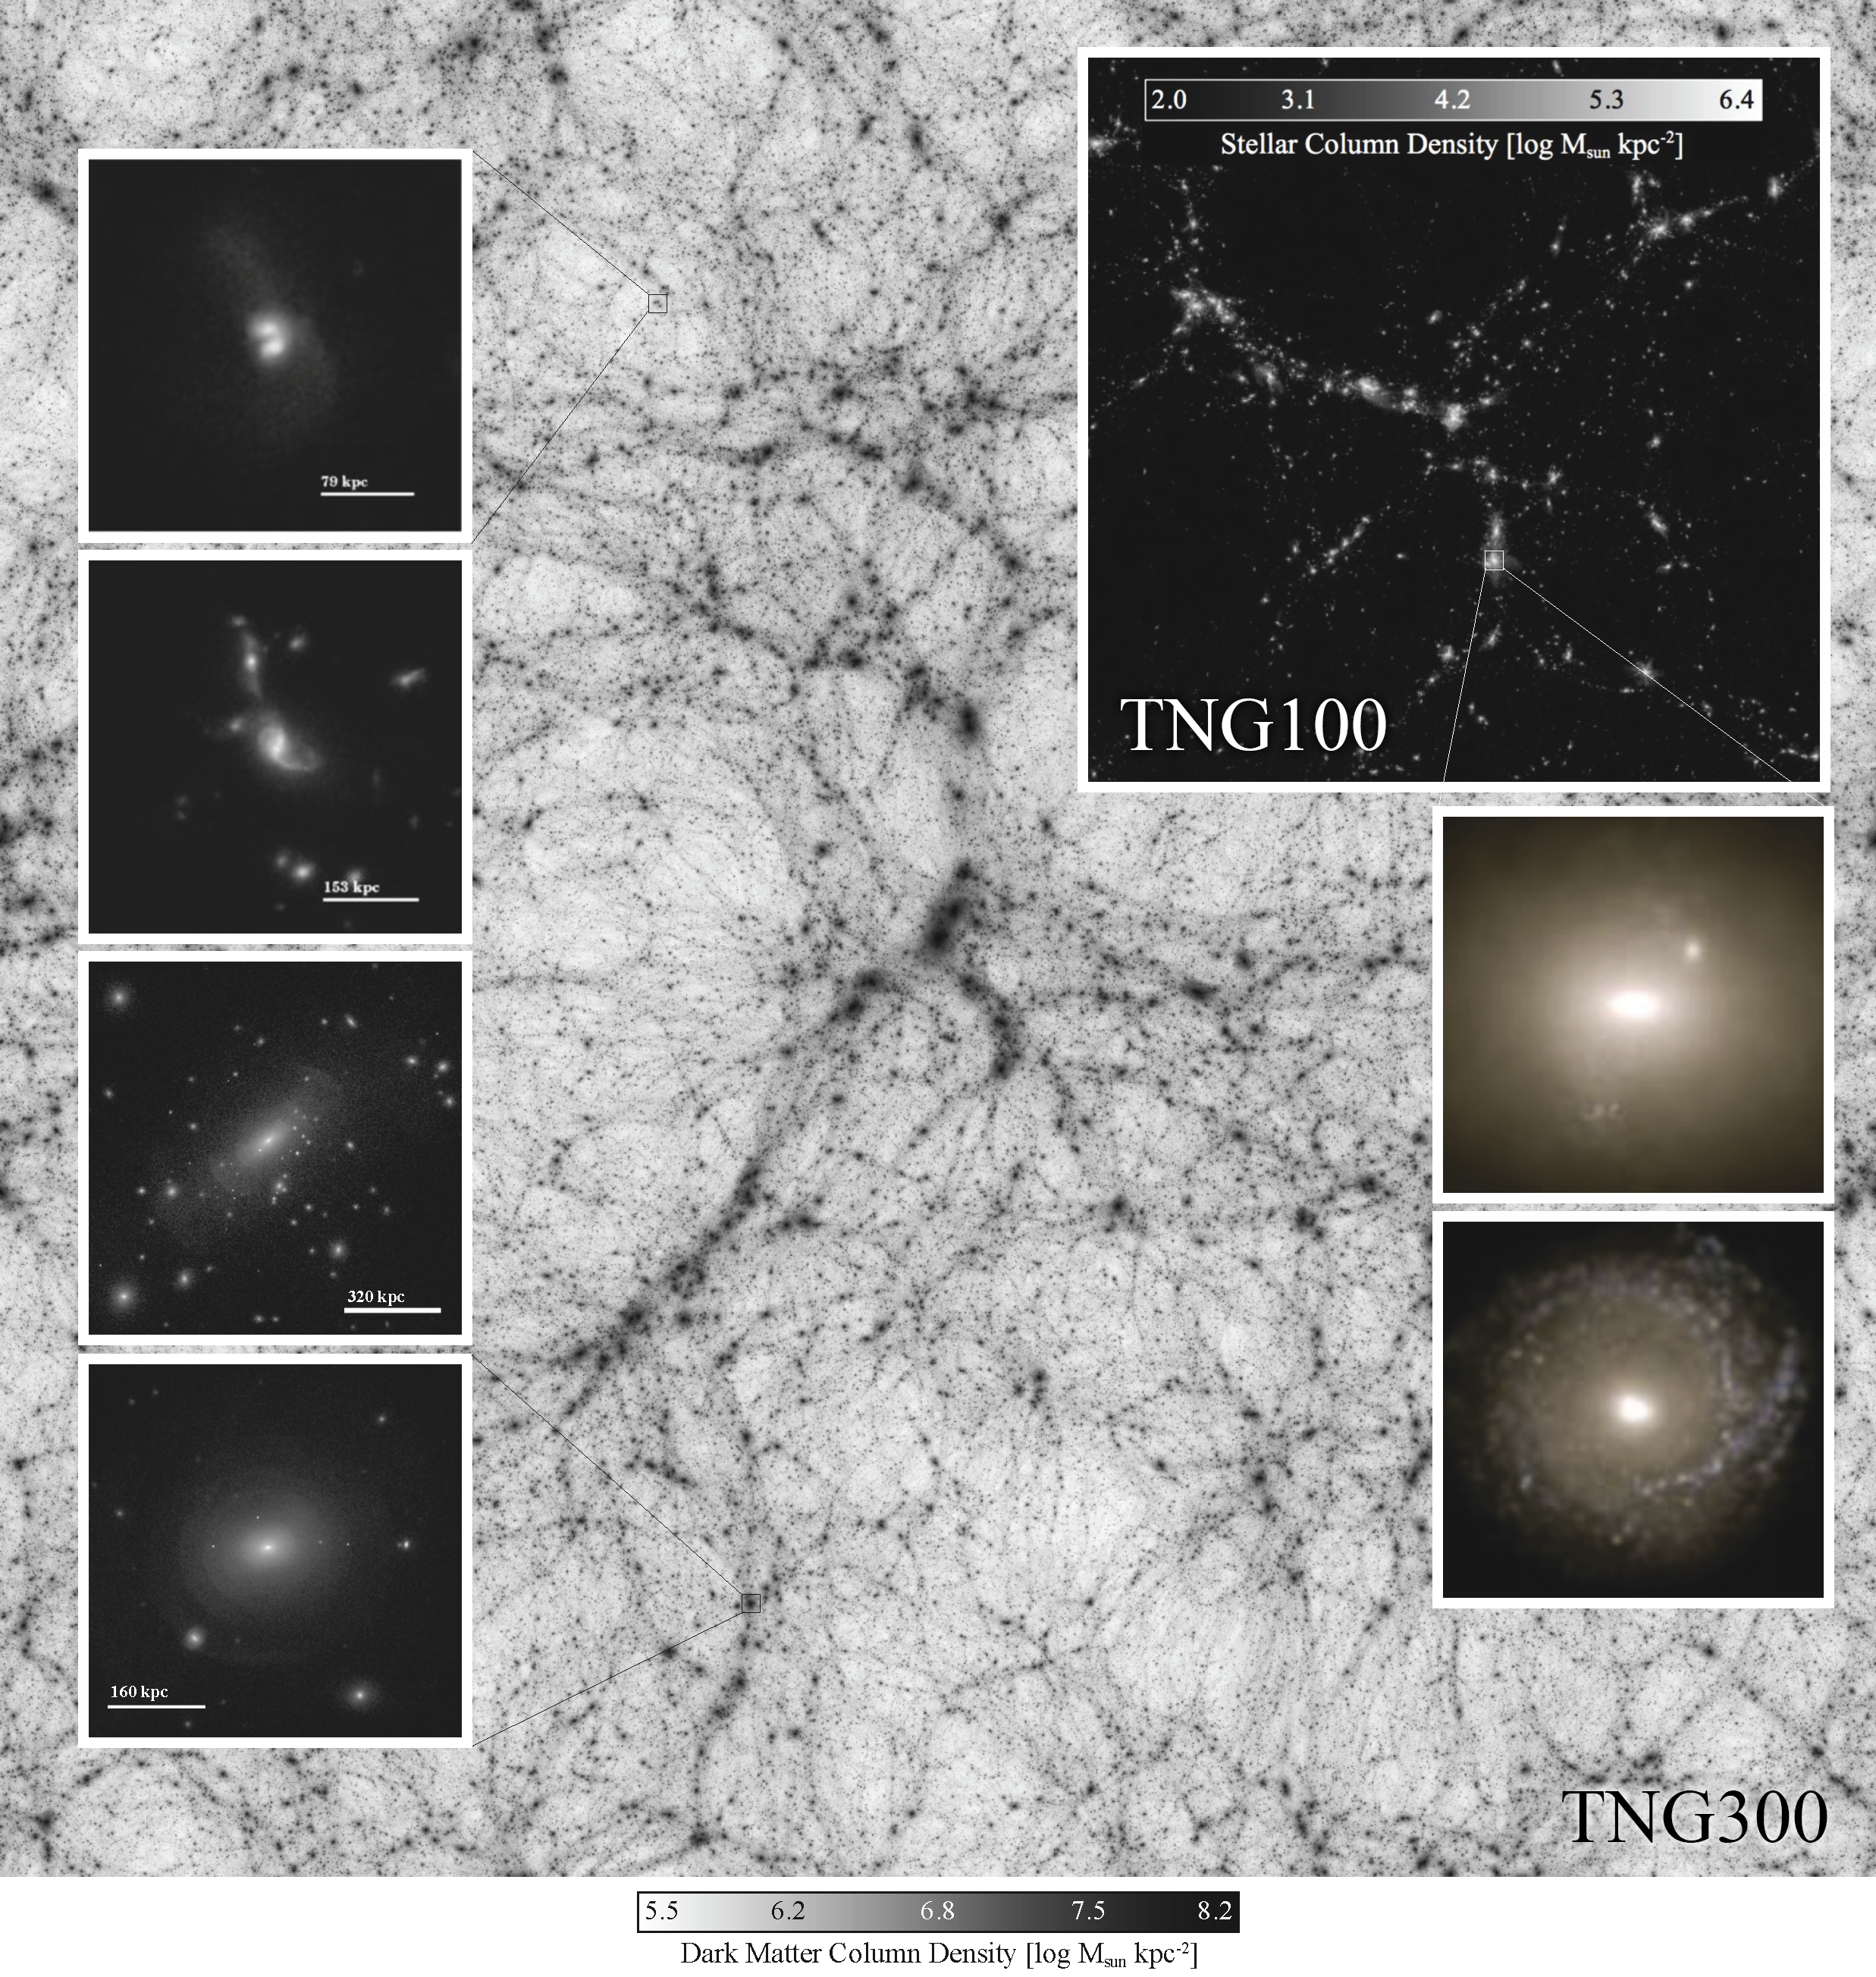
\includegraphics[width=0.9\textwidth]{images/TNG.png}
    \caption{A composite image that illustrates the two simulations TNG100 and TNG300. In the background is the dark matter distribution for the whole TNG300 volume. In the upper right is the stellar mass distribution across the entire TNG100 volume. The panels on the left show galaxy-galaxy interactions, while the panels on the right show the stellar light projections of two $z=0$ galaxies. Credit: TNG Collaboration}.
    \label{tng_illustration}
\end{figure}

\begin{table}
\begin{center}
\caption{The simulation details for the three main TNG simulations. $N_{DM}$ is the amount of dark matter particles. $m_{DM}$ and $m_{baryon}$ is the mass of the dark matter and baryonic particles, respectively.}
 \label{TNG}
\begin{tabular}{ l| c c c c c } 
 \hline
 \hline
   &  Volume [$Mpc^3$] & $N_{DM}$ & $m_{DM}$ [$M_{\odot}$] & $m_{baryon}$ [$M_{\odot}$] \\
 \hline
 TNG50 & $51.7^3$ & $2163^3$ & $4.5 \times 10^5 $ & $8.5 \times 10^4 $ \\ 
 TNG100 & $110.7^3$ & $1820^3$ & $7.5 \times 10^6 $ & $1.4 \times 10^6 $  \\ 
 TNG300 & $302.6^3$ & $2500^3$ & $5.9 \times 10^7 $ & $1.1 \times 10^7 $  \\ 
 \hline 
 \end{tabular}
\end{center}
\end{table}

\subsubsection{Data catalogs}
All the Illustris-TNG data is publically available online at the TNG webpage\footnote{https://www.tng-project.org/data/}. The data products that are available for each simulation are snapshots, group catalogs and merger trees as well as some supplementary data sets. There are five different particle types in the simulations, and each has its properties stored as particle fields. These fields include information like position, kinematic data and atomic/chemical composition. For each different run of the simulation, 100 snapshots are created, which are taken at specific redshifts. They include all the particles in the whole volume of the simulation, with 20 of them including all the fields for each particle as well.

The group catalogs provide a convenient way to quickly access already calculated properties of the different halos and subhalos instead of dealing with all the particles in a snapshot. This saves a lot of time and effort, but gives the user less control over what can be analyzed. There is one group catalog for each snapshot, and this includes two types of objects, Friends-of-Friends (FoF) and Subfind. The FoF catalog contains all the halos, and the Subfind catalog contains all the subhalos and their associated galaxy (if there is any) for each halo. Each subhalo has a parent halo, and the largest subhalo in each halo is the central subhalo. The merger trees data products contain the merger history of each subhalo.

This project makes use of the group catalogs and particles for the $z = 0$ snapshot.

\subsubsection{Sample reduction}

The TNG documentation recommends filtering out all subhalos that are flagged with the $SubhaloFlag$ field, and so these were cut from the data. These are most probably subhalos of non-cosmological origin, and so should not be considered real galaxies.

For the relations covered in this project, only the central galaxies in each halo are selected. The FoF catalog contains the index for the largest subhalo in each halo, so combining this information with the Subfind catalog allows one to create a subset of the data that contains only the central galaxies.

Only galaxies with stellar mass greater than $10^{9.5} M_{\odot}$ are used, which corresponds to about ?? stellar particles.

\subsection{Galaxy sizes}
When observing galaxies, we are looking at the luminosities from stars and gas. The detectors on instruments are limited, so there will always be a cut-off point at the faint end of the luminosity spectrum of a galaxy. Different apertures... //research//

In simulations we are not limited by instrumentations, attenuation and background light. However, a cut off point still needs to be determined. SUBFIND does this for the dark matter part of the simulation, seperating out subhalos from larger halos. The galaxy properties of that subhalo os then calculated using all the stellar and gas particles in the subhalo. When comparing simulation data to observational data, there are many ways to simulate the finite size of observed galaxies. Calculating luminosities and selecting a cut off point, using a physical aperture size (30 kpc for instance), using a multiple of the effective radius or using a fraction of the virial radius of the subhalo, to mention a few.

The stellar component of the galaxy is situated in the center of the dark matter halo, and usually extends out to about [...]. The (hot) gas compoenent of a galaxy is found in large amounts outside the stellar halo, so there might be a significant difference in the amount of gas based on which galaxy size is used.

\subsection{Galaxy properties}

\subsubsection{Magnitude and colors}
//Would be affected only by cut in radius.

The absolute magnitude ($\mathcal{M}$) is a measure of the total luminosity ($L$) of the galaxy such that $\mathcal{M} = -2.5 \log(L/L_\odot) + \mathcal{M}_\odot$, where $L_\odot$ is the solar luminosity and $\mathcal{M}_\odot$ is the solar magnitude.

For the TNG group catalog, the Subhalo field \texttt{SubhaloStellarPhotometrics} is used to get the magnitudes based on the summed up luminosities of all the stellar particles in the Subhalo. Eight bands are available, but in this work only the g- and i-band are used. The g-i colors are calculated by simply subtracting the i-band magnitude from the g-band magnitude.

\subsubsection{Masses}

\subsubsection{Size}
For the group catalog, the \texttt{SubhaloHalfmassRadStellar} field has been used. The half-mass radius is the radius of a spherical volume within which half the stellar mass is found. It is the 3D half-mass radius ($R_e$), as it is not a projected quantity.

\subsubsection{Velocities}

Galaxy velocities are for early and late type galaxies usually given by the velocity dispersion and rotational velocity, respectively. This is because of the shape of the two different galaxy types. It makes more sense to talk about velocity dispersion in a pressure dominated system and rotational velocity in a rotating disk.

//Rot vel: In TNG, the Subhalo field \texttt{SubhaloVMax} gives the maximum value for the spherically averaged rotation curve of a given galaxy. As the rotational curves are nearly flat for large enough radii, it should not be very important at which specific radius the observational rotational velocity is measured, as long as it is in the flat part of the curve. Accordingly, \texttt{SubhaloVMax} is used as the rotational velocity for the TNG data.

////////////

The velocity dispersion of a galaxy is the standard deviation of the line-of sight velocities.

\begin{equation} \label{standard_dev}
    \sigma^{2} = \frac{1}{N} \sum_{n=1}^{N} (V_{i} - \overline{V})^2
\end{equation}

In observations, the only velocities of the components of a galaxy we can measure are the line-of-sight velocities. These are calculated using the observed Doppler shift in the galactic spectrum. If the velocity dispersion tends to fall off at larger radii, and the galaxy has an ellipsoid shape, the angle at which the galaxy is viewed will have an effect on the observed velocity dispersion. To compensate for this, velocity dispersions in simulations may be calculated in three different projections of the galaxy and averaged over these. 

\begin{equation} \label{sigma1}
    \sigma^{2} = \frac{1}{3}(\sigma_x^2 + \sigma_y^2 + \sigma_z^2)
\end{equation}

This has been done by calculating the velocity dispersion within the projected half-mass radius in each projection.


In SUBFIND, the velocity dispersion is simply calculated as the velocity dispersion of all the particles over the entire subhalo. This would naturally lead to lower values as the particles further out have lower velocities. Also, the velocities of the dark matter is something which cannot be taken into account in observations.


\subsection{Galaxy morphology classifications}

An important factor in many studies of galaxy formation and evolution is looking at and comparing the properties of the two morphological populations of galaxies. As an actual visual classification is intensively time consuming, other methods have been devised for identifying early and late type galaxies in simulations. In many studies, several of these classification criteria are used in conjunction.

\subsubsection{Gas fraction}
As early type galaxies have much less cold gass than late type galaxies, a simple cut in the galaxy population based on gas fraction will be effective at seperating the two types. As TNG doesn't differentiate between cold and hot gas, it is important then to consider the physical volume where the gas fraction is calculated. A large volume will enevitably contain more hot gas, and potentially allow for early type galaxies to be considered as late types. Late type galaxies also have a wide range of gas fractions. The most masssive spiral galaxies can contain as little as 5\% gas, while low-mass disks can contain up to 80\% \parencite{Mo2010}. In //Ferrero2020 galaxies with less than 10\% gas were considered for early types, while those with more were potential candidates for late type classifications. 

\subsubsection{Star formation rate}
Another way of seperating galaxies into the early and late-type categories is by using the specific star formation rate (sSFR). In this case, the galaxies are tagged as ``quenched'' and ``main-sequence'', where quenched galaxies have little to no star formation, while main-sequence galaxies have a significant amount of star formation. More formally, they are divided by how far from the ridge of the star-formation main-sequence they are found. In \cite{Genel2017} the ridge og the main-sequence is defined as the mean of the sSFR for galaxies with mass $10^{9} M_{\odot} < M_* < 10^{10.5} M_{\odot}$, and takes a value of $\log (sSFR[Gyr^{-1}]) = -0.94$ for $z=0$. Galaxies are then `main-sequence' if their sSFR are within 0.5 dex of this value. ``Quenched'' galaxies are defined as those with sSFR at least 1 dex below the ridge.

\subsubsection{Rotational kinetic energy}
A common way of estimating a galaxy's ``diskyness'' is to use the rotational-to-total-kinetic-energy parameter $\kappa_{rot}$. This value gives an indication of how much of the kinetic energy of the galaxy is invested in the ordered rotation about its axis. To calculate $\kappa_{rot}$, the axis of rotation must first be found. This is, in the case of a disk galaxy, simply the direction of the mass-averaged angular momentum of the inner parts of the galaxy. For an elliptical galaxy this ``rotation-axis'' would just be a random direction. The galaxy is then rotated such that the z-axis is pointed towards the axis of rotation, and $kappa_{rot}$ may be found.
\begin{equation}
    \kappa_{rot} = \frac{K_{rot}}{K} = \frac{\sum_{i=1}^{N} m_i (j_{z, i}/R_i)^2}{\sum_{i=1}^{N} m_i v_i^2},
\end{equation}
where $j_{z, i}$ is the z-component of the specific angular momentum ($\vec{j} = \vec{r} \times \vec{v}$) of particle $i$, $m_i$ is the mass of stellar particle $i$, and $R_i$ is the projected radius of stellar particle $i$ in the xy-plane. For a perfect disk galaxy that is totally rotationally supported $\kappa = 1$, while for a totally pressure supported system, $\kappa$ would approach zero. In //Sales2012, galaxies were classified as early type if they had $\kappa_{rot} < 0.5$ and late type for $\kappa_{rot} > 0.7$. This leads to a significant amount of ``intermediate types'', so other works have simply made a single cut at $\kappa_{rot} = 0.6$.